\documentclass[12pt]{report}
\usepackage [left=25.4mm,top=25.4mm]{geometry}
\usepackage{amsmath}
\usepackage{amssymb}
\usepackage{graphicx}
\usepackage{apacite}
\usepackage{url}
\usepackage{subfig}
\usepackage{csvsimple}
\usepackage{float}
\usepackage{tikz}

\begin{document}
\begin{titlepage}
\title{Pseudocode for MRPC Update}
\author{ Jarred M. Kvamme \\ University of Idaho \\ Department of Statistical Science }
\maketitle
\end{titlepage}

\newcommand{\indep}{\perp \!\!\! \perp}


\section*{1.1 The Trio Specific Case:}



In a network consisting of three nodes: $G( V, T_1, T_2)$ we can identify the 5 possible topologies laid out under MRPC using results of the coefficient tests from the pair of regressions on each non-instrumental variable (Please refer to the \textbf{Appendix} at the end for Tables, Figures, and mathematical definitions).\\

we preform two regressions using each non-intrumental variable node $T_i$ as the response once to yield the pair of linear models:

\begin{eqnarray}
T_1 = \beta_0 +\beta_{11}V+\beta_{21}T_2+{\bf \Gamma U}+ \epsilon \\
\nonumber\\
T_2 = \beta_0 +\beta_{21}V+\beta_{22}T_1+{\bf \Gamma U}+ \epsilon 
\end{eqnarray}

we also estimate and test the marginal relationship between $V$ and $T_2$. Let

\[ \hat{r} = \frac{\text{cov}(V,T_2)}{\hat{\sigma}_V \hat{\sigma}_{T_2}} \]

we can obtain the hypothesis test

\[ H_0: r = 0 \ \ \ H_A: r \neq 0 \]

which after use of the Fisher transformation

\[  F(\hat{r}) = \frac{1}{2}\ln\left(\frac{1+\hat{r}}{1-\hat{r}}\right) \]

approximates a normal distribution asymptotically in the sample size with parameters

\[  \text{mean} = F(r) \ \text{and SE} = \frac{1}{\sqrt{n-3}}\]

therefore by standardizing we have 

\[ Z_{\text{obs}} = \frac{F(\hat{r}) - F(r_0)}{SE} = \frac{\sqrt{n-3}}{2}\ln\left(\frac{1+\hat{r}}{1-\hat{r}}\right) \approx N(0,1) \]

where we 

\[ \text{reject $H_0$ if} \ \ \ 2\times P(Z>|Z_{\text{obs}}|)<\alpha \]

where $r_0$ denotes the correlation under the null hypothesis and $F(r_0)$ is zero.\\
\\

Combining the results of the tests for all $\beta_{ij}$ regression coefficients from the models above and the marginal test defined above, we can determine the topology of the network (see \textbf{Table 1} in \textbf{Appendix})

\subsection*{1.2 - Permuted Regression for Rare Variants} - We will apply the permuted regression described by Yang et al., 2017 whenever the instrumental variable contains a rare count at frequency $< \gamma$. The permuted regression is preformed to obtain a robust estimate of the mediation effect between $T_i$ and $T_j$ in $G(V, T_i, T_j)$ which may be masked in the standard regression when $V$ contains few observations for the minor variant. The algorithm for preforming the permuted regression is as follows:\\
\\
\begin{quote}
\textbf{step 1.} - Let $f_{\text{minor}}$ be the frequency of the minor variant of $V$. If $f_{\text{minor}} < \gamma$ preform the permuted regression(s) else preform the standard regression(s).
\end{quote}

\begin{quote}
\textbf{step 2.} - repeat $m$ times: permute $T_2$ in $\bf (1)$ within the levels of $V$ denoted $T_2^{\ast}$. Similarly, permute $T_1$ in $\bf (2)$ within the levels of $V$ denoted $T_1^{\ast}$. Next preform the regressions using the permuted variables:

\begin{eqnarray}
T_1 = \beta_0 +\beta_{11}V+\beta_{21}^{\ast}T_2^{\ast}+{\bf \Gamma U}+ \epsilon \\
\nonumber\\
T_2 = \beta_0 +\beta_{21}V+\beta_{22}^{\ast}T_1^{\ast}+{\bf \Gamma U}+ \epsilon \nonumber 
\end{eqnarray}

\end{quote}


\begin{quote}
\textbf{Step 3.} - Let $\bf \Theta_{21}$ and $\bf \Theta_{22}$ denote $(m \times 1)$ vectors representing the collection of $T$ statistics from the wald tests on $\beta_{21}^{\ast}$ and $\beta_{22}^{\ast}$ coefficients (respectively) from the permuted regressions in \textbf{Step 2.}. such that:

\[ {\bf \Theta}_{21} = \left[ T_{21}^{\ast (1)}, \ T_{21}^{\ast (2)}, \ T_{21}^{\ast (3)}, \cdots \right] \]

\[ {\bf \Theta}_{22} = \left[ T_{22}^{\ast (1)}, \ T_{22}^{\ast (2)}, \ T_{22}^{\ast (3)}, \cdots \right]  \]

We next test the association between $T_1$ and $T_2$ using the nominal test defined by Yang et. al., 2017. Let $T_{\text{obs}_{21}}$ be the observed wald statistic from $\bf (1)$ and $T_{\text{obs}_{22}}$ be the observed wald statistic from $\bf(2)$. We formulate the testable hypotheses: 

\[ H_0: T_{\text{obs}_{21}} = \mu_{21}^{\ast}, \ \ H_A: T_{\text{obs}_{21}} \neq \mu_{21}^{\ast} \]
and
\[ H_0: T_{\text{obs}_{22}} = \mu_{22}^{\ast}, \ \ H_A: T_{\text{obs}_{22}} \neq \mu_{22}^{\ast} \]

where $\mu_{21}^{\ast}$ and $\mu_{22}^{\ast}$ denote the centers of the non-central $T$ distributions of $\bf \Theta_{21}$ and $\bf \Theta_{22}$ respectively. Therefore the mediation test statistic is:

\[ Z_{\text{obs}_{ij}} = \frac{T_{\text{obs}_{ij}} - \frac{\sum {\bf \Theta}_{ij}}{m} }{SE({\bf \Theta}_{ij})} \]

where we 

\[ \text{reject $H_0$ if} \ \ \ 2\times P(Z >  |Z_{\text{obs}_{ij}}|) < \alpha \]

\end{quote}



\section*{2. General Algorithm}

\textbf{Step 1.} - Starting with a fully connected graph of $p+1$ nodes, compute the precision matrix of the data: \\
Assuming $\bf X$ is centered:

\[ X \sim N_k({\bf 0}, \bf{\Sigma})  \ \ \ \text{for} \ k=p+q+1\]
 
Then the precision matrix of $\bf X$ is defined as 

\[  {\bf H} = {\bf \Sigma}^{-1} \]

$\bf H$ can be scaled to the partial correlation matrix for the entries in $\bf X$. Given the entry in the $i^{th}$ row and $j^{th}$ column of $\bf H$:

\[  {\bf x}_i, {\bf x}_j | {\bf x}_{-(i,j)} = - \frac{h_{ij}}{\sqrt{h_{ii}}\sqrt{h_{jj}}} = \hat{\rho}_{\bf x_i,x_j\cdot x_{ -(i,j)}  }\]

which is a measure of the association between the $i^{th}$ and $j^{th}$ columns/variables in $\bf X$ conditioned on all other variables. \\
\\
The Fisher transformation can be used to formulate a test for each partial correlation coefficient of interest:

\[ \frac{\sqrt{n - |{\bf x_{-i,j}}| -3}}{2}\ln\left( \frac{1+\hat{\rho}_{\bf x_i,x_j\cdot x_{ -(i,j)}  }}{1-\hat{\rho}_{\bf x_i,x_j\cdot x_{ -(i,j)}  }} \right)  \approx N(0,1)\]

where null and alternative hypotheses are 
\[ H_0:  \hat{\rho}_{\bf x_i,x_j\cdot x_{ -(i,j)}  } = 0 \ \ \ H_A: \hat{\rho}_{\bf x_i,x_j\cdot x_{ -(i,j)}  }\neq 0\]

\[  \text{reject $H_0$ if} \ \  | Z_{\text{obs}}| > Z_{1-\alpha/2 }\]

by applying the cases:

\[  a_{i,j} = \begin{cases}1 & \text{if} \ \ P(Z>Z_{\text{obs}})<\alpha \\
                                      0 & \text{else} 
  \end{cases} \ \ \forall i,j \in 1:p+1\]

we can obtain the $(p+1 \times p+1)$ adjacency matrix $\bf A$ for the network skeleton\\


The use of the partial correlations matrix has been shown to be applicable for the construction of an undirected acyclic graph (insert references here). We suggest here to use the partial correlation network obtained from \textbf{Step 1.} to construct the graph skeleton\\


\noindent \textbf{Step 2.} - Determine the directed structure of all $p\choose 2$ possible 3-node networks involving the instrumental variable(s) using the regressions and tests outlined in \textbf{Section 1.}. Here we are breaking up the structure of the larger network into trios of nodes involving the instrumental variable i.e all $G(V, T_i, T_j) \ \forall i\neq j$\\

\begin{quote}
\textbf{Step 2.1} - (Specific to Genomics) if the minor variant frequency (allele frequency or copy number variation) of the instrumental variable $V$ is less than the predetermined threshold $i.e < \gamma$, preform the permuted regression described in \textbf{Section 1.2}. 
\end{quote}

\noindent \textbf{Step 3.} -  Determine the directed structure of all $p\choose 3$ possible 3-node networks involving only the non-instrumental variable nodes using the regressions and tests outlined in \textbf{Section 1.}. This step is to find edges that may be explained away when conditioning on other nodes in the network. i.e we infer all possible $G(T_i, T_j, T_k) \ \forall i\neq j\neq k$\\












\newpage
\section*{Appendix}
\begin{quote}
\textbf{Definitions}\\
$V$ - The instrumental variable\\
$T_i$ - a non-instrumental variable/node\\
$p$ - the number of non-instrumental variables/nodes in a network\\
$q$ - the number of confounding variables selected for a network\\
$m$ - the number of permutations to preform in a permuted regression (mediation test)\\
$n$ - the sample size of the data\\
$\bf U$ - the $(n \times q)$ matrix whose columns represent confounding variables\\
$\bf X$ - the $(n \times p+q+1)$ data matrix of all variables/nodes and all confounders\\
$\bf H$ - the $(p+q+1 \times p+q+1)$ precision matrix \\
$A$ - a $(p+1 \times p+1)$ adjacency matrix for the network  \\
$G(A,B,C)$ - a graph with nodes A, B, and C\\
$F(\cdot)$ - the Fisher transformation function\\
$\gamma$ - the minimum frequency for which we would preform  permuted regression is needed\\
$\rho_{\bf x_i,x_j\cdot x_{ -(i,j)}  }$ - the partial correlation between the $i^{th}$ and $j^{th}$ columns/variables of ${\bf X}$
\end{quote}

\begin{table}[H]
\centering
\caption{ Expected results for the tests on the regression coefficients under each model scenario }
\begin{tabular}{|c||cccc|c|}
\hline
\bf Model  & $\bf\beta_{11}$  &  $\bf\beta_{21}$   & $\bf\beta_{12}$    & $\bf\beta_{22}$    & $ V \indep T_2$    \\ \hline \hline
\bf M0      &  $= 0$                & $\neq 0$              & $=0$                    & $=0$                    & Yes  \\ \hline 
               &  $= 0$                & $= 0$                  & $=0$                    & $\neq 0$               & No       \\ \hline
\bf M1      &  $\neq 0$            &  $\neq 0$             & $\neq0$                & $ = 0$                 & No  \\ \hline
\bf M2      &   $\neq0$            &  $\neq 0$             & $\neq0$                & $\neq0$               & Yes  \\ \hline
\bf M3      &   $=0$                &  $\neq 0$             & $=0$                    & $\neq0$               & Yes  \\ \hline
\bf M4      &   $\neq0$            &  $\neq 0$             & $\neq0$                & $\neq0$               & No  \\ \hline
\end{tabular}
\end{table}

\begin{figure}[H]
\begin{center}
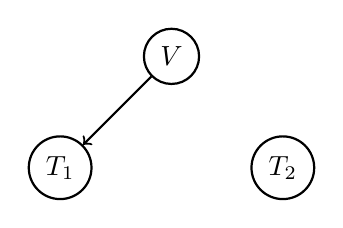
\begin{tikzpicture}[node distance={20mm}, thick, main/.style = {draw, circle}] 
\node[main] (1) {$V$};
\node[main] (2) [below left of=1] {$T_1$};
\node[main] (3) [below right of=1] {$T_2$} ;
\draw[->] (1) -- (2);
\end{tikzpicture}
\end{center}
\caption{M0 - $V\not\indep T_1 ; V \indep T_2; T_1 \indep T_2$ }
\end{figure}


\begin{figure}[H]
\begin{center}
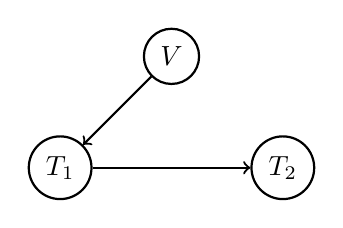
\begin{tikzpicture}[node distance={20mm}, thick, main/.style = {draw, circle}] 
\node[main] (1) {$V$};
\node[main] (2) [below left of=1] {$T_1$};
\node[main] (3) [below right of=1] {$T_2$} ;
\draw[->] (1) -- (2);
\draw[->] (2) -- (3);
\end{tikzpicture}
\end{center}
\caption{M1 - $V\not\indep T_1 ; V \not\indep T_2; T_1 \not\indep T_2; V \indep T_2 | T_1$}
\end{figure}

\begin{figure}[H]
\begin{center}
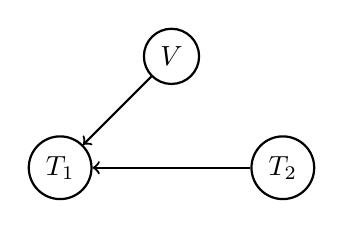
\begin{tikzpicture}[node distance={20mm}, thick, main/.style = {draw, circle}] 
\node[main] (1) {$V$};
\node[main] (2) [below left of=1] {$T_1$};
\node[main] (3) [below right of=1] {$T_2$} ;
\draw[->] (1) -- (2);
\draw[<-] (2) -- (3);
\end{tikzpicture}
\end{center}
\caption{M2 - $ V\not\indep T_1 ; V \indep T_2; T_1 \not\indep T_2; V \not\indep T_2 |T_1 $}
\end{figure}

\begin{figure}[H]
\begin{center}
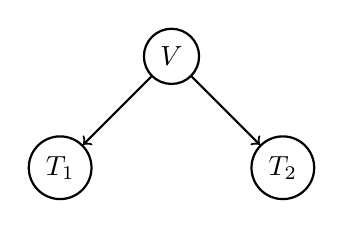
\begin{tikzpicture}[node distance={20mm}, thick, main/.style = {draw, circle}] 
\node[main] (1) {$V$};
\node[main] (2) [below left of=1] {$T_1$};
\node[main] (3) [below right of=1] {$T_2$} ;
\draw[->] (1) -- (2);
\draw[->] (1) -- (3);
\end{tikzpicture}
\end{center}
\caption{fig: M3 - $V\not\indep T_1 ; V \not\indep T_2; T_1 \not\indep T_2; T_1 \indep T_2 | V$}
\end{figure}

\begin{figure}[H]
\begin{center}
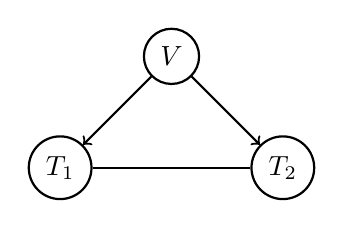
\begin{tikzpicture}[node distance={20mm}, thick, main/.style = {draw, circle}] 
\node[main] (1) {$V$};
\node[main] (2) [below left of=1] {$T_1$};
\node[main] (3) [below right of=1] {$T_2$} ;
\draw[->] (1) -- (2);
\draw[->] (1) -- (3);
\draw (2) -- (3);
\end{tikzpicture}
\end{center}
\caption{fig: M4 - $V\not\indep T_1 ; V \not\indep T_2; T_1 \not\indep T_2; T_1 \not\indep T_2 | V$}
\end{figure}






































































\end{document}